\section{Question 4}
ISS spacecraft observation orbital elements and Ground Station Location location is provided in \ref{table:orbital-elements}, and \ref{table:lat-long}, respectively. The orbital elements are used to calculate the position of the ISS spacecraft at the time of observation. The position is then used to calculate the line of sight vector from the ground station to the ISS spacecraft. The line of sight vector is then used to calculate the elevation and azimuth angles of the ISS spacecraft. The elevation and azimuth angles are then used to calculate spacecraft visibility.
\begin{table}[H]
    \centering
    \label{table:orbital-elements}
    % \vspace{.2cm}
    \Tstrut
    \begin{tabular}{|c|c|}
    \hline
    Orbital Element & Value \\
    \hline
    Eccentricity & 0.0005771 \\
    Inclination & \ang{51.6409} \\
    Perigee Height & 415km \\
    Apogee Height & 423km \\
    RAAN & \ang{88.8414} \\
    Argument of Perigee & \ang{75.2083} \\
    True Anomaly & 0 \\
    \hline
    \end{tabular}
    \caption{ISS Observation}
\end{table}

\begin{table}[H]
    \centering
    \label{table:lat-long}
    \begin{tabular}{|c|c|}
    \hline
    Latitude & Longitude \\
    \hline
    \ang{34}13'28.9''N & \ang{118}03'26.3''W \\
    \hline
    \end{tabular}
    \caption{Ground Station Location}
\end{table}

\begin{figure}[H]
    \centering
    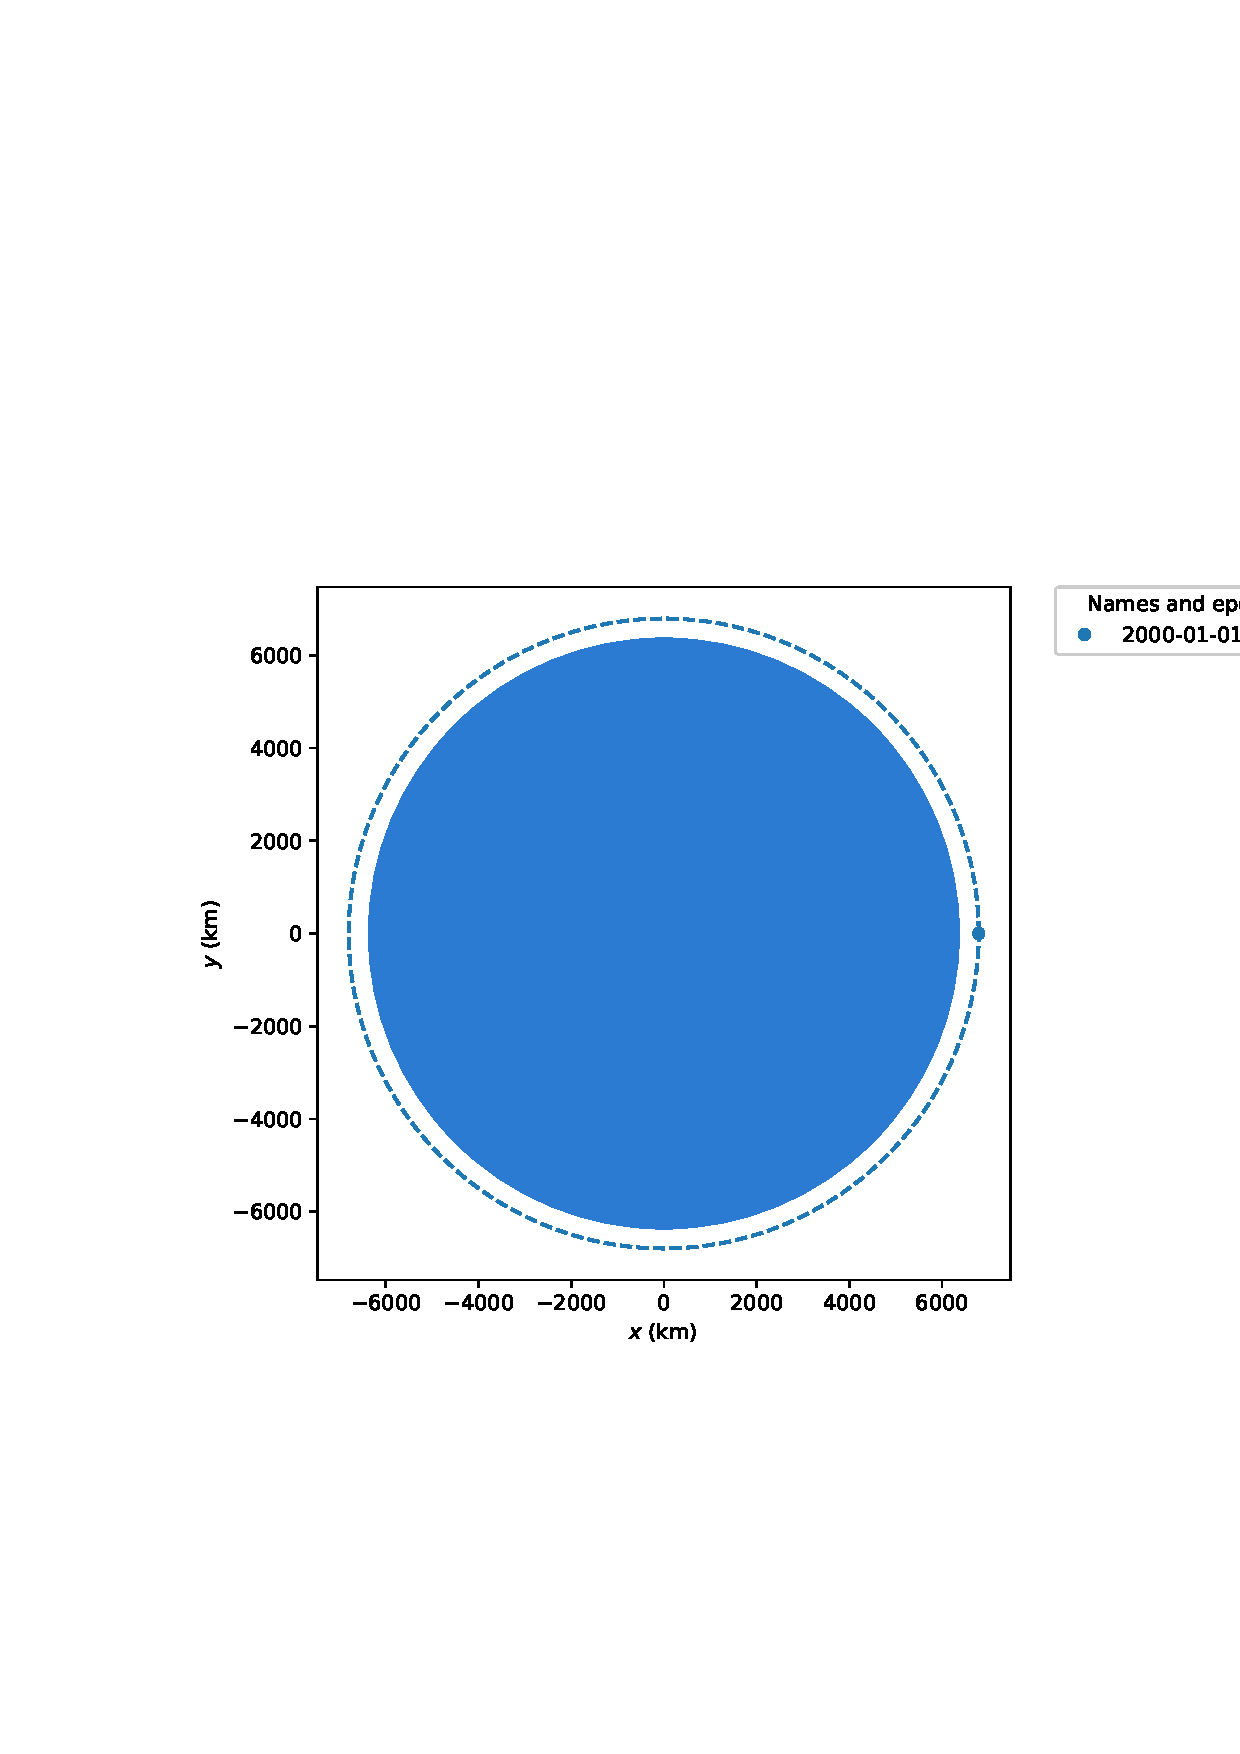
\includegraphics[width=\textwidth]{../Figure/Q4/orbiral.png}
    \caption{ISS spacecraft orbit.}
    \label{fig:ISS_orbit}
\end{figure}

\subsection{part a}
The spacecraft differential equations were solved for 48 hours to find the position of the ISS spacecraft at the time of observation in GCRF. The result is shown in \ref{fig:ISS_orbit_GCRF}.

\begin{figure}[H]
    \centering
    \includegraphics[width=\textwidth]{../Figure/Q4/GCRF.png}
    \caption{ISS spacecraft orbit in GCRF.}
    \label{fig:ISS_orbit_GCRF}
\end{figure}

\subsection{part b}
The position of the ISS spacecraft at the time of observation in GCRF is then converted to ITRF with 
 function in Q4.ipynb Jupyter notebook.
The result is shown in \ref{fig:ISS_orbit_ITRF}.

\begin{figure}[H]
    \centering
    \includegraphics[width=\textwidth]{../Figure/Q4/ITRF.png}
    \caption{ISS spacecraft orbit in ITRF.}
    \label{fig:ISS_orbit_ITRF}
\end{figure}

\subsection{part c}
In this part of the homework, we used the Astropy coordinate library to calculate the line of sight vector from a ground station to the International Space Station (ISS) spacecraft. To determine if the spacecraft is visible, we calculated the attitude and azimuth and checked if the elevation angle is greater than \ang{10}. The implementation of this algorithm can be found in the Q4.ipynb Jupyter Notebook.

Our calculations showed that the spacecraft is visible for a total of 169,351 seconds, which is equivalent to 48 hours. We used a step time of 1 second in our calculations.

\subsection{part d}
In this section, we implemented the above algorithm to calculate the visibility of the International Space Station (ISS) for all latitudes from \ang{-90} to \ang{90} and longitudes from \ang{-180} to \ang{180}. After performing the calculations, we found that the location with the most observation time is:

[Insert coordinates and location information here]
This information can be useful for planning future observations of the ISS. We performed these calculations using a step time of 1 minute and a step size of 30 degrees for both latitudes and longitudes. This level of granularity allowed us to obtain accurate results while minimizing computational time.
The best location for the ground station is at latitude \ang{-30.00} degrees and longitude \ang{-60.00} degrees, with a total view time of 47.15 hours over the 48 hours.
\begin{table}[H]
    \centering
    \label{table:lat-long}
    \begin{tabular}{|c|c|}
    \hline
    Latitude & Longitude \\
    \hline
    \ang{-30}N & \ang{-60}W \\
    \hline
    \end{tabular}
    \caption{Ground Station Location}
\end{table}